\documentclass[12pt, aspectratio=43]{beamer}
\usepackage[backend=bibtex, style=authoryear]{biblatex} % bibliography
\usepackage{multirow}
\usepackage{adjustbox}

% BEAMER TEMPLATE AND THEME
\setbeamertemplate{footline}[frame number]
\usetheme{Estonia}
\mode<presentation>
\AtBeginSection[]{
  \begin{frame}
  \vfill
  \centering
  \begin{beamercolorbox}[sep=8pt,center,shadow=true,rounded=true]{title}
    \usebeamerfont{title}\insertsectionhead\par%
  \end{beamercolorbox}
  \vfill
  \end{frame}
}

\addbibresource{../biblio.bib}

% TITLE PAGE
\title{Kubernetes cluster simulator based on Batsim}
\title{Development and evaluation of a Kubernetes cluster simulator based on
Batsim}

\author{\textbf{Presented by:} Théo Larue\\\textbf{Supervised by:} Olivier
Richard \& Michael Mercier}

\date{August 31, 2020}

\institute[Théo LARUE]{Université Grenoble Alpes}

\titlegraphic{
	
\includegraphics[height=5ex]{../imgs/uga-logo.png}\hspace{2ex}
	
\includegraphics[height=6ex]{../imgs/ENSIMAG.png}\hspace{2ex}
	
\includegraphics[height=5ex]{../imgs/Logo-LIG.jpg}\hspace{2ex}
	
\includegraphics[height=5ex]{../imgs/ryax-logo.png}
}

\begin{document}

\frame{\titlepage}

\begin{frame}\frametitle{Table of contents}\tableofcontents
\end{frame}

\section{Introduction}
\begin{frame}{Computer infrastructures}
	\uncover<1->{
		\textit{A distributed system is a system whose components are
		located on different networked computers, which communicate and
	coordinate their actions by passing messages to one another.}
	\footnote{\cite{andrew2002tanenbaum}}
	}

	\uncover<2->{
		\begin{exampleblock}{Many domains}
			Grid, Edge, HPC, Cloud, P2P, Volunteer.
		\end{exampleblock}
	}
\end{frame}

\begin{frame}[allowframebreaks]{Studying distributed systems}
	\centering
	Why studying these infrastructures?
	%Why studying these infra? To test a system performances under varying
	%loads, applications, scheduling policies, system size and topology. Or
	%to develop new RJMS or research new scheduling algorithms.
	
	\framebreak
	TODO
	One problem in particular: scheduling.
\end{frame}

\begin{frame}{Different approches}
	\uncover<1->{
		\begin{block}{How to study these infra?}
			\begin{itemize}
					\uncover<2->{\item Theoretical study.}
					\uncover<3->{\item Real experiments.}
					\uncover<4->{\item Emulation.}
					\uncover<5->{\item Simulation.}
			\end{itemize}
		\end{block}
	}
	%How to study these infra? Too many elements and interactions to
	%consider, so no theoretical study. 

	%Real experiments are too costly (both in time and resources) and not
	%reproducible.

	%Note: revoir ref sur les interactions inattendues entre scheduler et
	%queues 
\end{frame}

\section{Literature review}
\begin{frame}{Domain specific simulators}
	refs on domain specific simulators, summed up in a table. Explain
	briefly the concept behind some of them.
\end{frame}

\begin{frame}{Software specific simulators}
	YARNSim, SLURM simulator
\end{frame}

\begin{frame}{Publication specific simulators}
	``Publish and perish'' - Milian Poquet
\end{frame}

\begin{frame}{SimGrid}
	SimGrid: Versatile, scalable, accurate.

	Cpu = a computation speed.\\
	Storage = a seek time and a data transfert rate.\\
	Network = a flow model, modeling bandwith sharing behaviors.

	Simple models but thoroughly validated.
\end{frame}

\begin{frame}{Batsim}
	Aimed at studying RJMS.

	Strong decoupling decision process / simulator.
\end{frame}

\begin{frame}{Batsim - related work}
	Alea: modular, extensible.

	Accasim: supports additional information (temperature, power
	consuption). Very efficient in terms of simulation time and memory
	usage.

	Both outperform Batsim in terms of scalability. However it is not fair
	to compare them on this point because Batsim relies on well thought
	models, when these two only implement delay jobs.
\end{frame}

\begin{frame}{Kubernetes}
	Explain containers real quick.

	Container orchestration software, description based.
\end{frame}

\begin{frame}{Kubernetes cluster simulation}
	k8s-cluster-simulator: open source, student project, delay jobs.
	Schedulers provided via a Go interface.

	joySim: closed-source, fully fledged kubernetes cluster simulator,
	service oriented (mock nodes).
\end{frame}

\section{Integrating Kubernetes schedulers to Batsim}

\begin{frame}{Technical challenges}
	\begin{alertblock}{Challenges to tackle}
		\begin{enumerate}
				\uncover<1->{\item Integration with Kubernetes.}
				\uncover<2->{\item Intercepting scheduler time.}
				\uncover<3->{\item Time synchronization between Batsim and the scheduler.}
		\end{enumerate}
	\end{alertblock}
\end{frame}

\begin{frame}{Batsim concepts}
	\begin{columns}
		\column{0.5\textwidth}
		\centering
		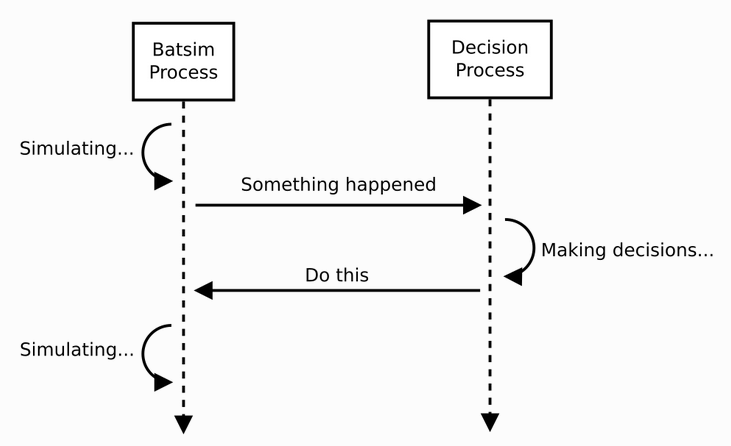
\includegraphics[width=\textwidth]{../imgs/batsim-sequence-diag.png}
		\tiny{source \url{https://batsim.readthedocs.io}}

		\column{0.5\textwidth}
		Batsim events and protocol.

		User defined workloads.

		(insert json examples?)
\end{columns}
\end{frame}

\begin{frame}{Kubernetes concepts}
	\centering
	\only<1>{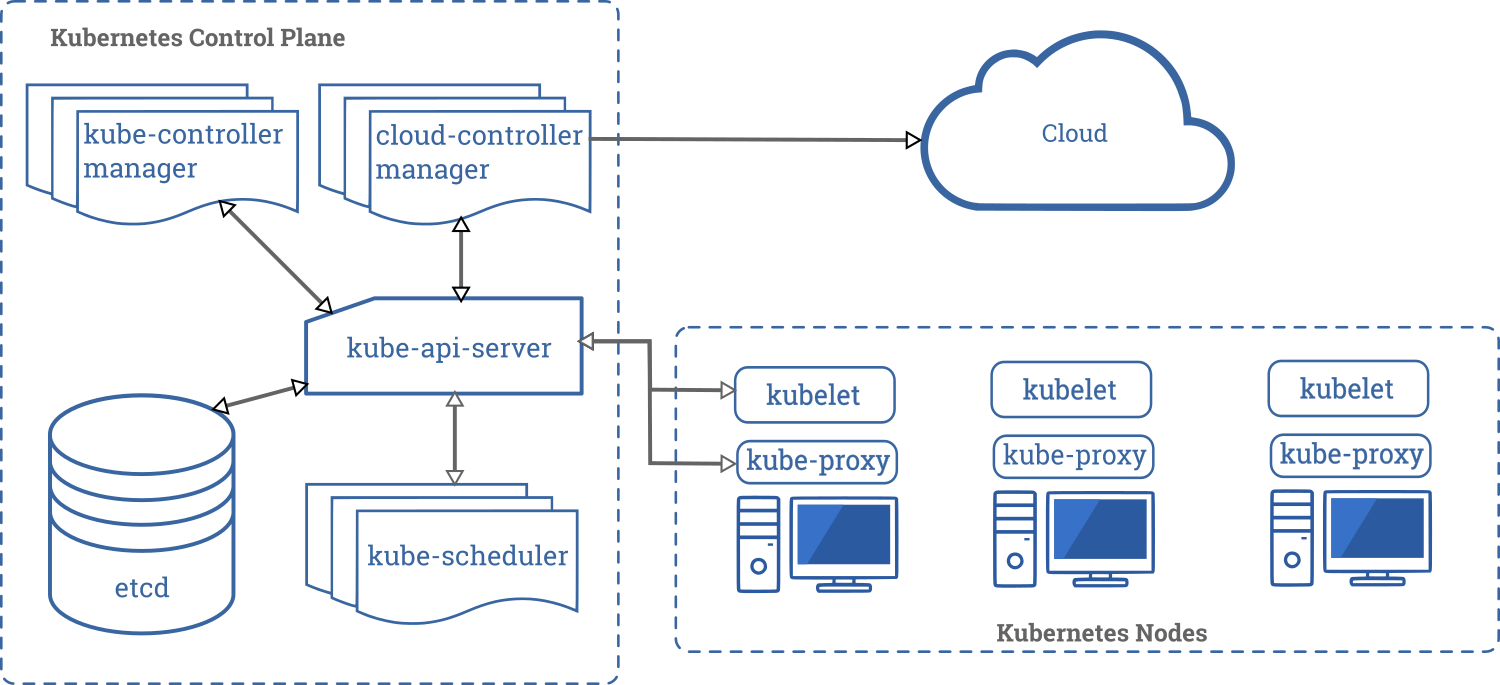
\includegraphics[width=\textwidth]{../imgs/components-of-kubernetes.png}}
	\only<2>{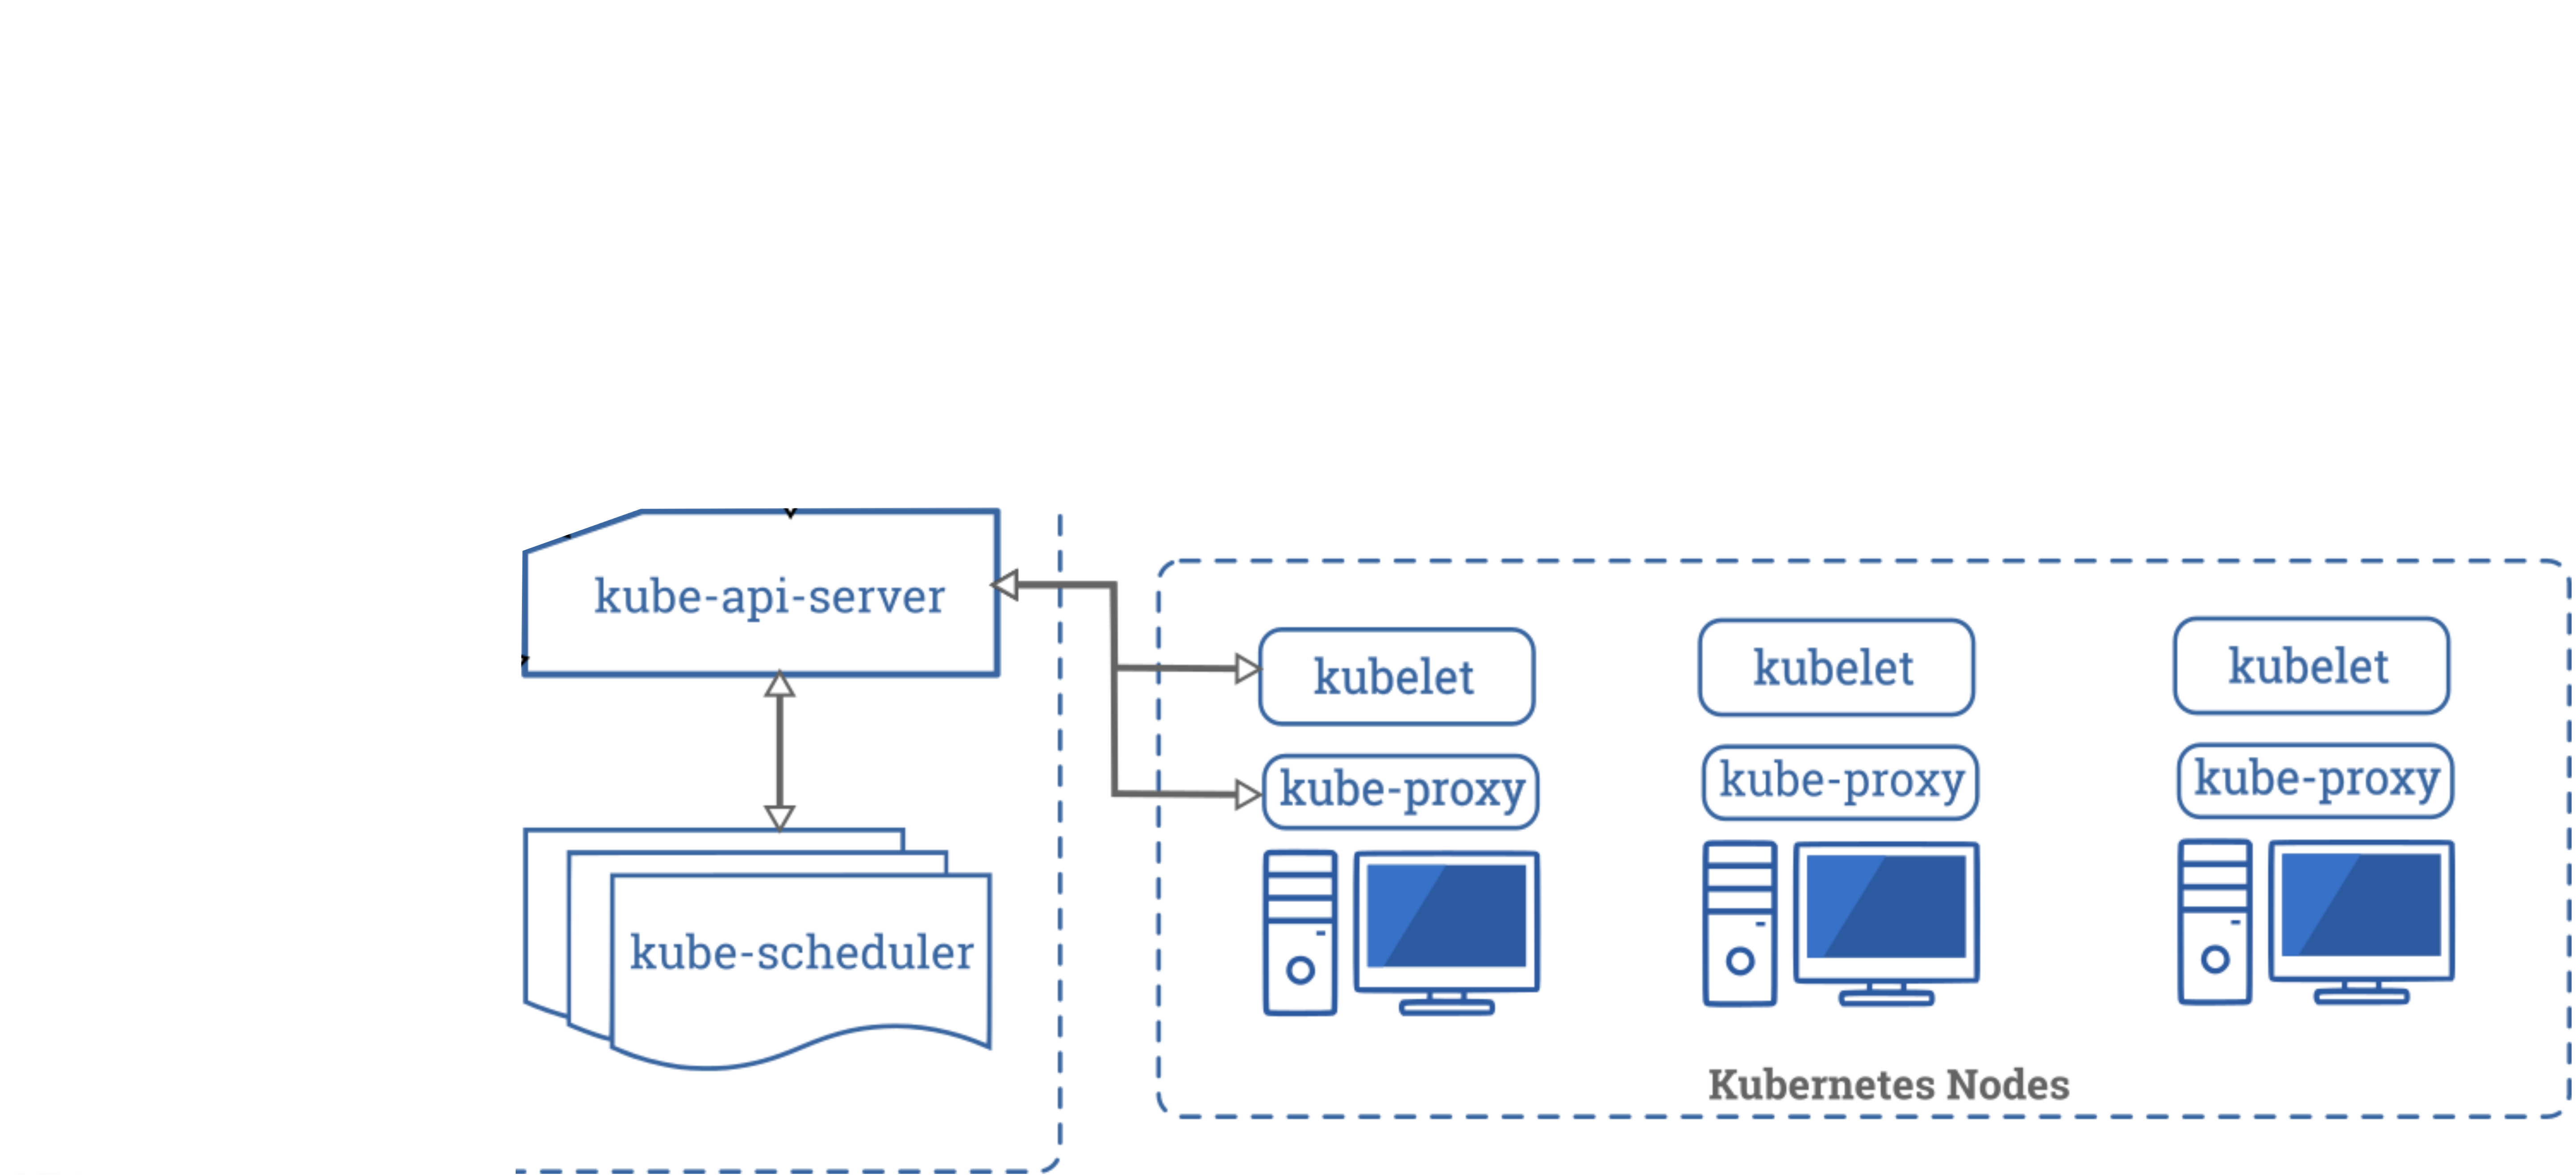
\includegraphics[width=\textwidth]{../imgs/components-of-kubernetes-2.png}}
	\tiny{source: \url{https://kubernetes.io/docs/concepts/overview/components/}}\\
	\small{Kubernetes components.}
\end{frame}

\begin{frame}{Different paradigms}
	Batsim: event based, simulation time.

	Kubernetes scheduler: asynchronous calls to the API, machine time.

	The goal is to make the scheduler event based and relying on simulation
	time for Batsim, and make Batsim a kube-api-server to the scheduler.
\end{frame}

\begin{frame}{Batkube integration with Kubernetes}
	\centering
	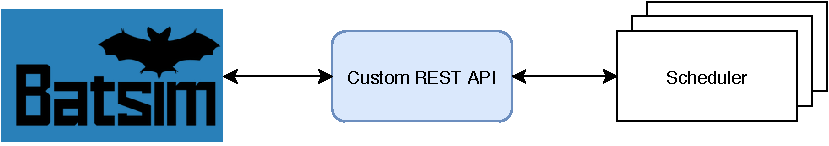
\includegraphics[width=0.8\textwidth]{../imgs/custom-api.pdf}\\
	\small{Reimplementation of a custom API.}
\end{frame}

\begin{frame}{Architeture of Batkube}
	\centering
	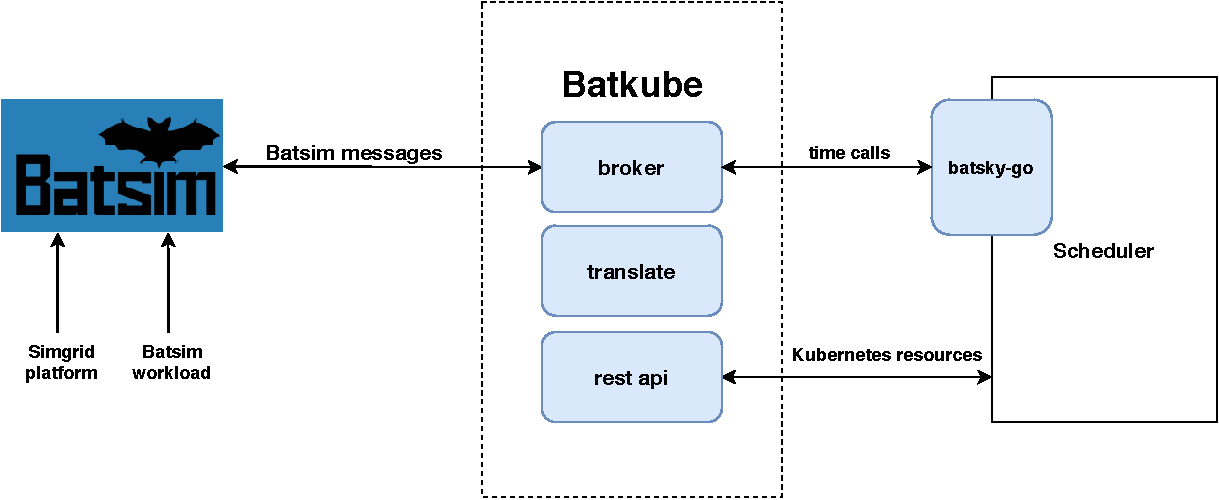
\includegraphics[width=\textwidth]{../imgs/batkube-architecture-3-synchro.pdf}
	\small{Global architecture of Batkube.}
\end{frame}


\begin{frame}{Similar resources}
	\begin{columns}
		\column{0.5\textwidth}
		\centering
		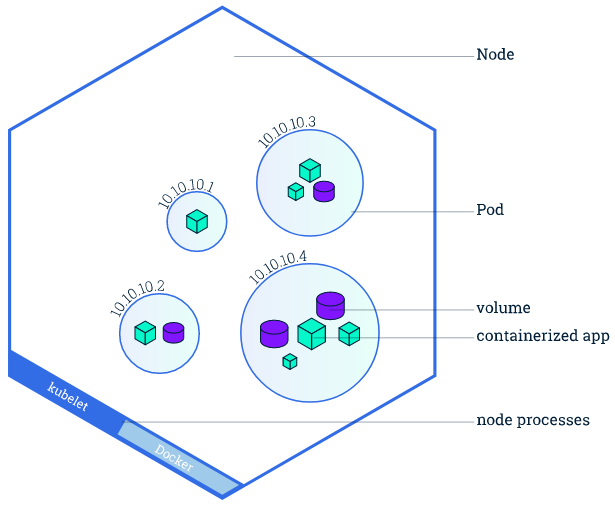
\includegraphics[width=\textwidth]{../imgs/node-overview.png}
		\tiny{source: \url{https://kubernetes.io/docs/tutorials/kubernetes-basics/explore/explore-intro/}}

		\column{0.5\textwidth}
		\begin{block}{Translation between Kubernetes and Batsim}
			\begin{itemize}
				\item A Pod = a job.
				\item A Node = a compute resource.
			\end{itemize}
		\end{block}
	\end{columns}
\end{frame}

\begin{frame}{Time interception}
	\centering
	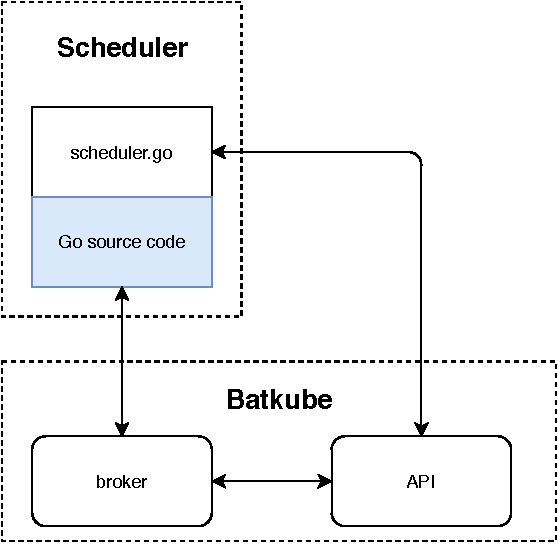
\includegraphics[width=0.6\textwidth]{../imgs/synchro-go-sources.pdf}\\
	\small{Schedulers are patched to redirect their time.}
\end{frame}

\begin{frame}{batsky-go}
	\begin{columns}
		\column{0.5\textwidth}
		\centering
		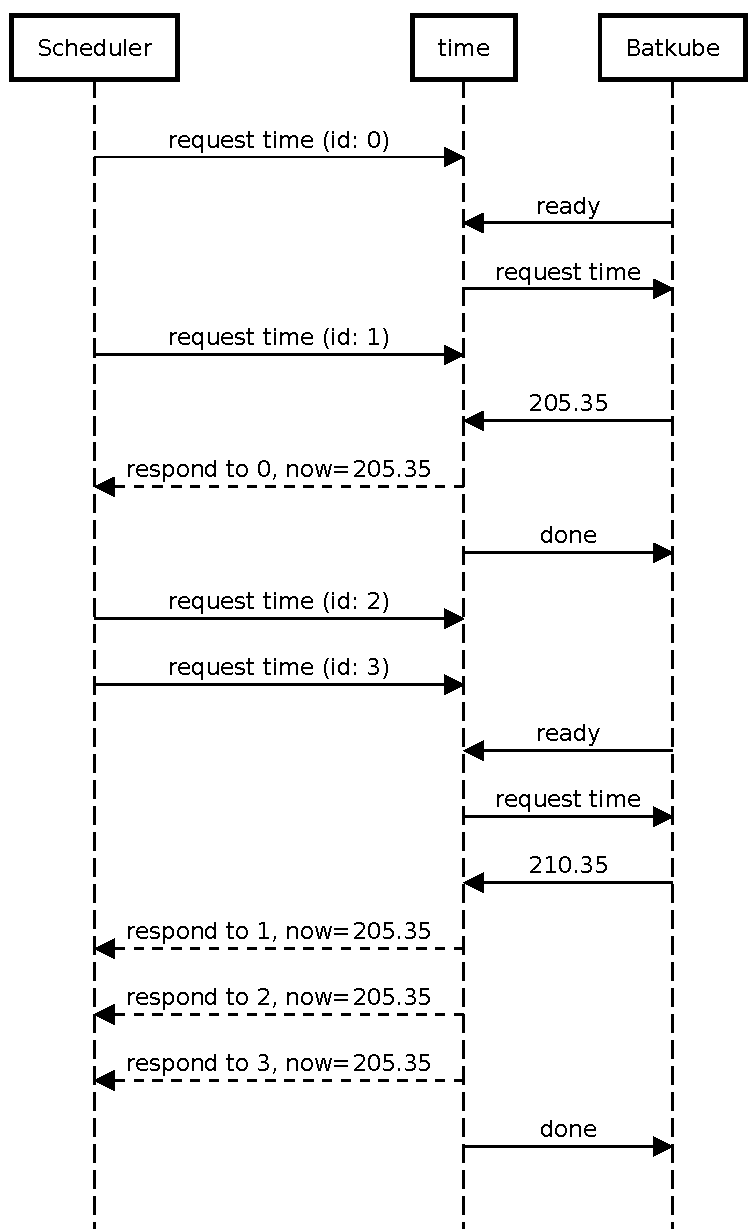
\includegraphics[scale=0.38]{../imgs/requester-broker.pdf}
		
		\column{0.5\textwidth}
		Exchanges between the scheduler, batsky-go (``time'') and Batsim
	\end{columns}
\end{frame}

\begin{frame}[allowframebreaks]{Time synchronization}
	TODO: explain CML
	\framebreak

	\centering
	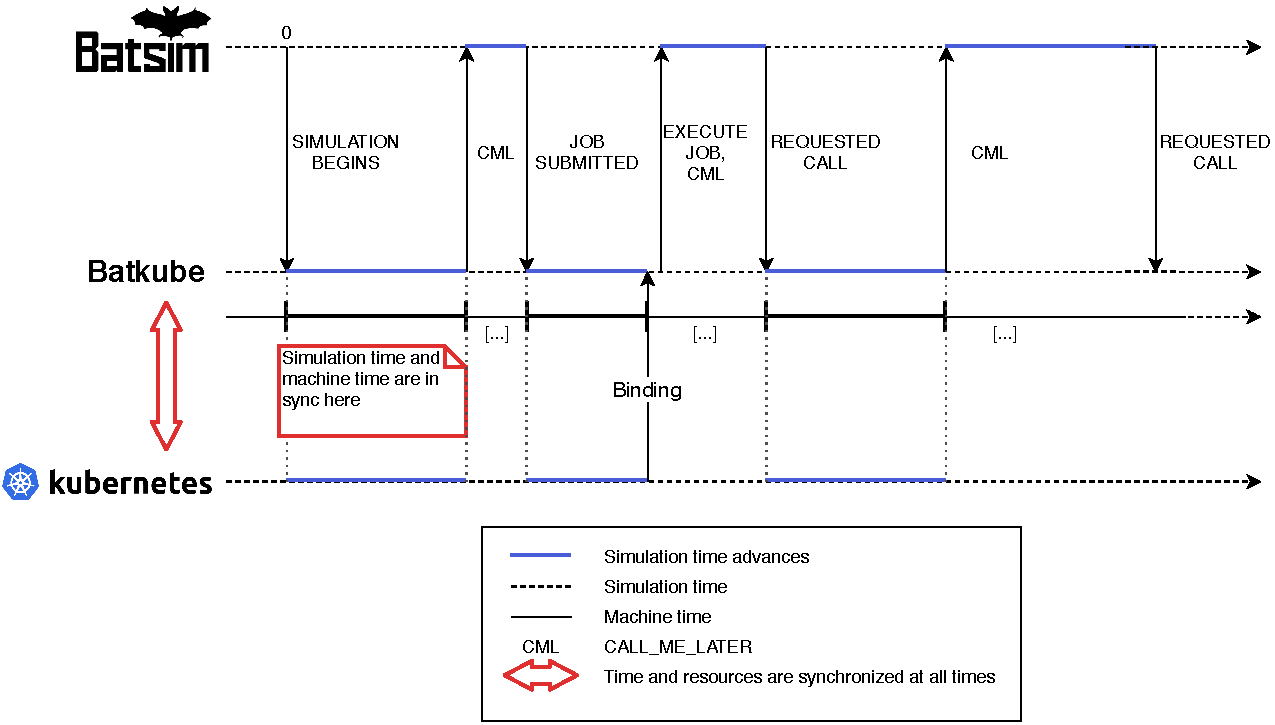
\includegraphics[width=0.87\textwidth]{../imgs/lignes_de_temps_simple.pdf}\\
	\small{Time synchronization between Batsim and the scheduler}
\end{frame}

\begin{frame}{Parameters of the synchronization}
	\only<1>{
		\centering
		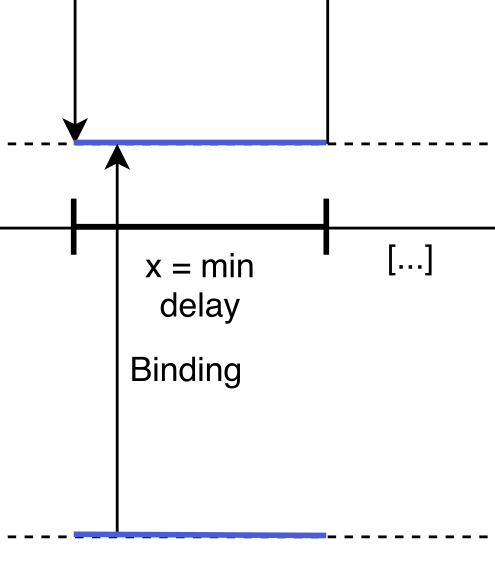
\includegraphics[scale=0.3]{../imgs/min-delay.png}\\
		Minimum delay
	}
	\only<2>{
		\centering
		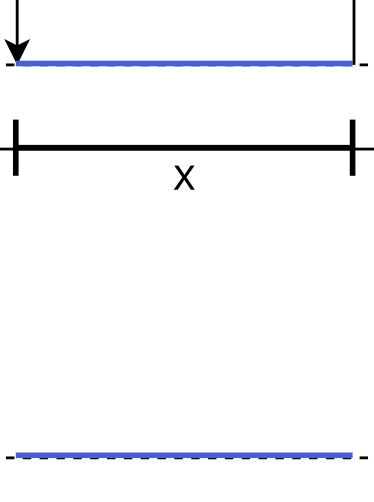
\includegraphics[scale=0.3]{../imgs/timeout.png}\\
		Timeout value
	}
	\only<3>{
		\centering
		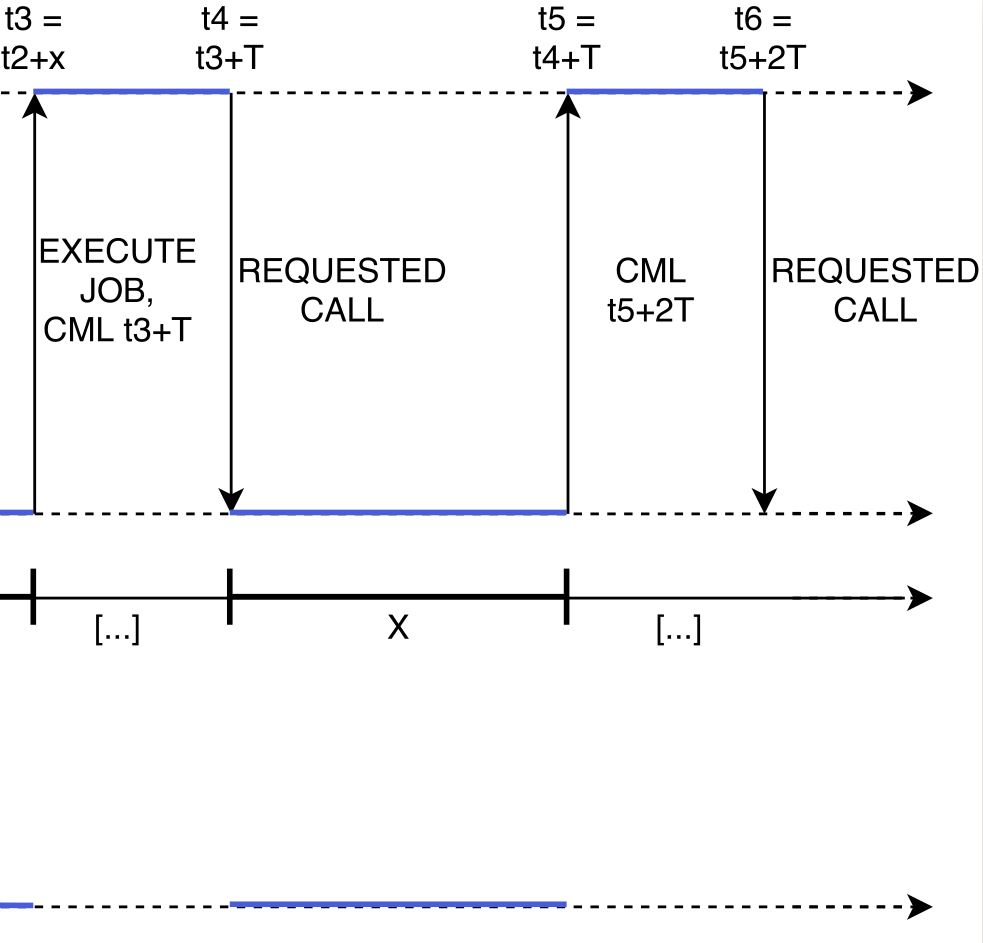
\includegraphics[scale=0.2]{../imgs/max-timestep.png}\\
		Simulation time step $\in$ [\texttt{base-simulation-timestep}, \texttt{max-simulation-timestep}]
	}
\end{frame}

\begin{frame}{Time synchronization breakdown}
	\centering
	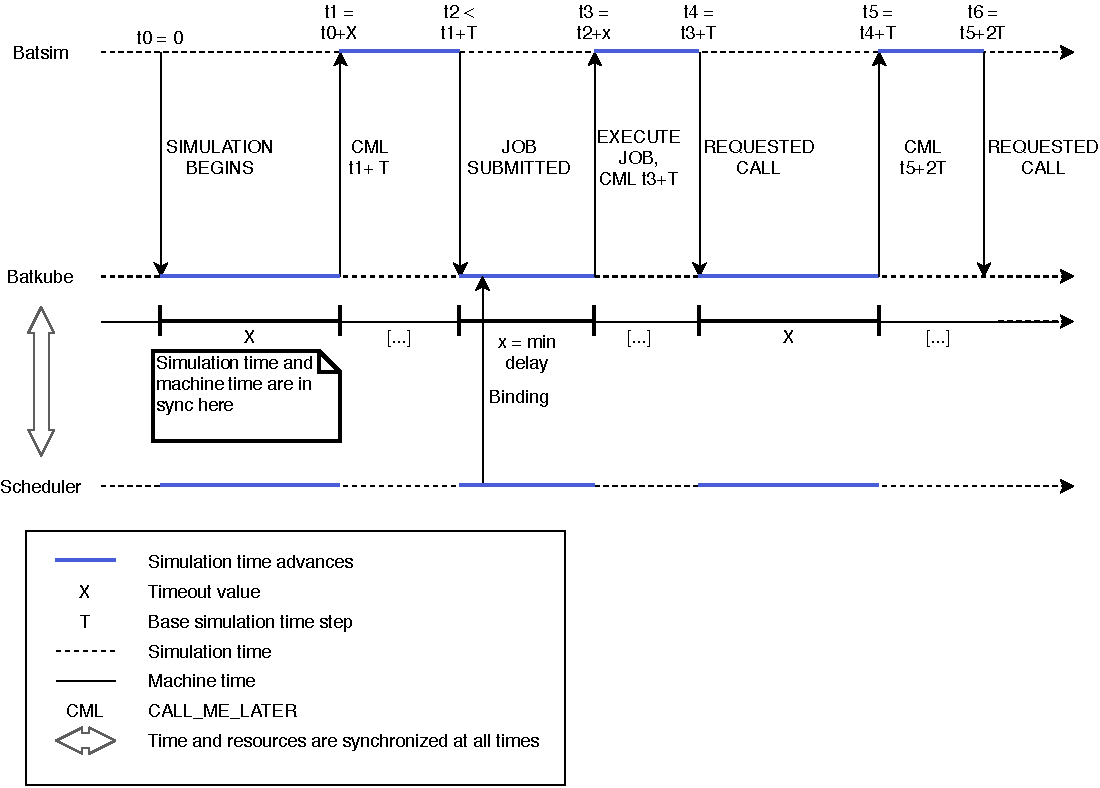
\includegraphics[width=0.87\textwidth]{../imgs/lignes_de_temps.pdf}\\
	\small{Time synchronization between Batsim and the scheduler}
\end{frame}

\section{Study of the simulator}
\begin{frame}{Studied workloads and platforms}
	TODO
	%\centering
	%\begin{tabular}{|c|c|c|c|c|c|}
	%	\hline\\
	%	name & number of jobs & jobs type & sub time & resource requests & platform
	%	\hline\\
	%	burst & 200 & delay (170s) & at time zero & 1 cpu & 16x1\\
	%	spaced & 200 & delay (170s) & every ten seconds & 1 cpu & 16x1\\
	%\end{tabular}
\end{frame}

\begin{frame}[allowframebreaks]{Minimum delay}
	\centering
	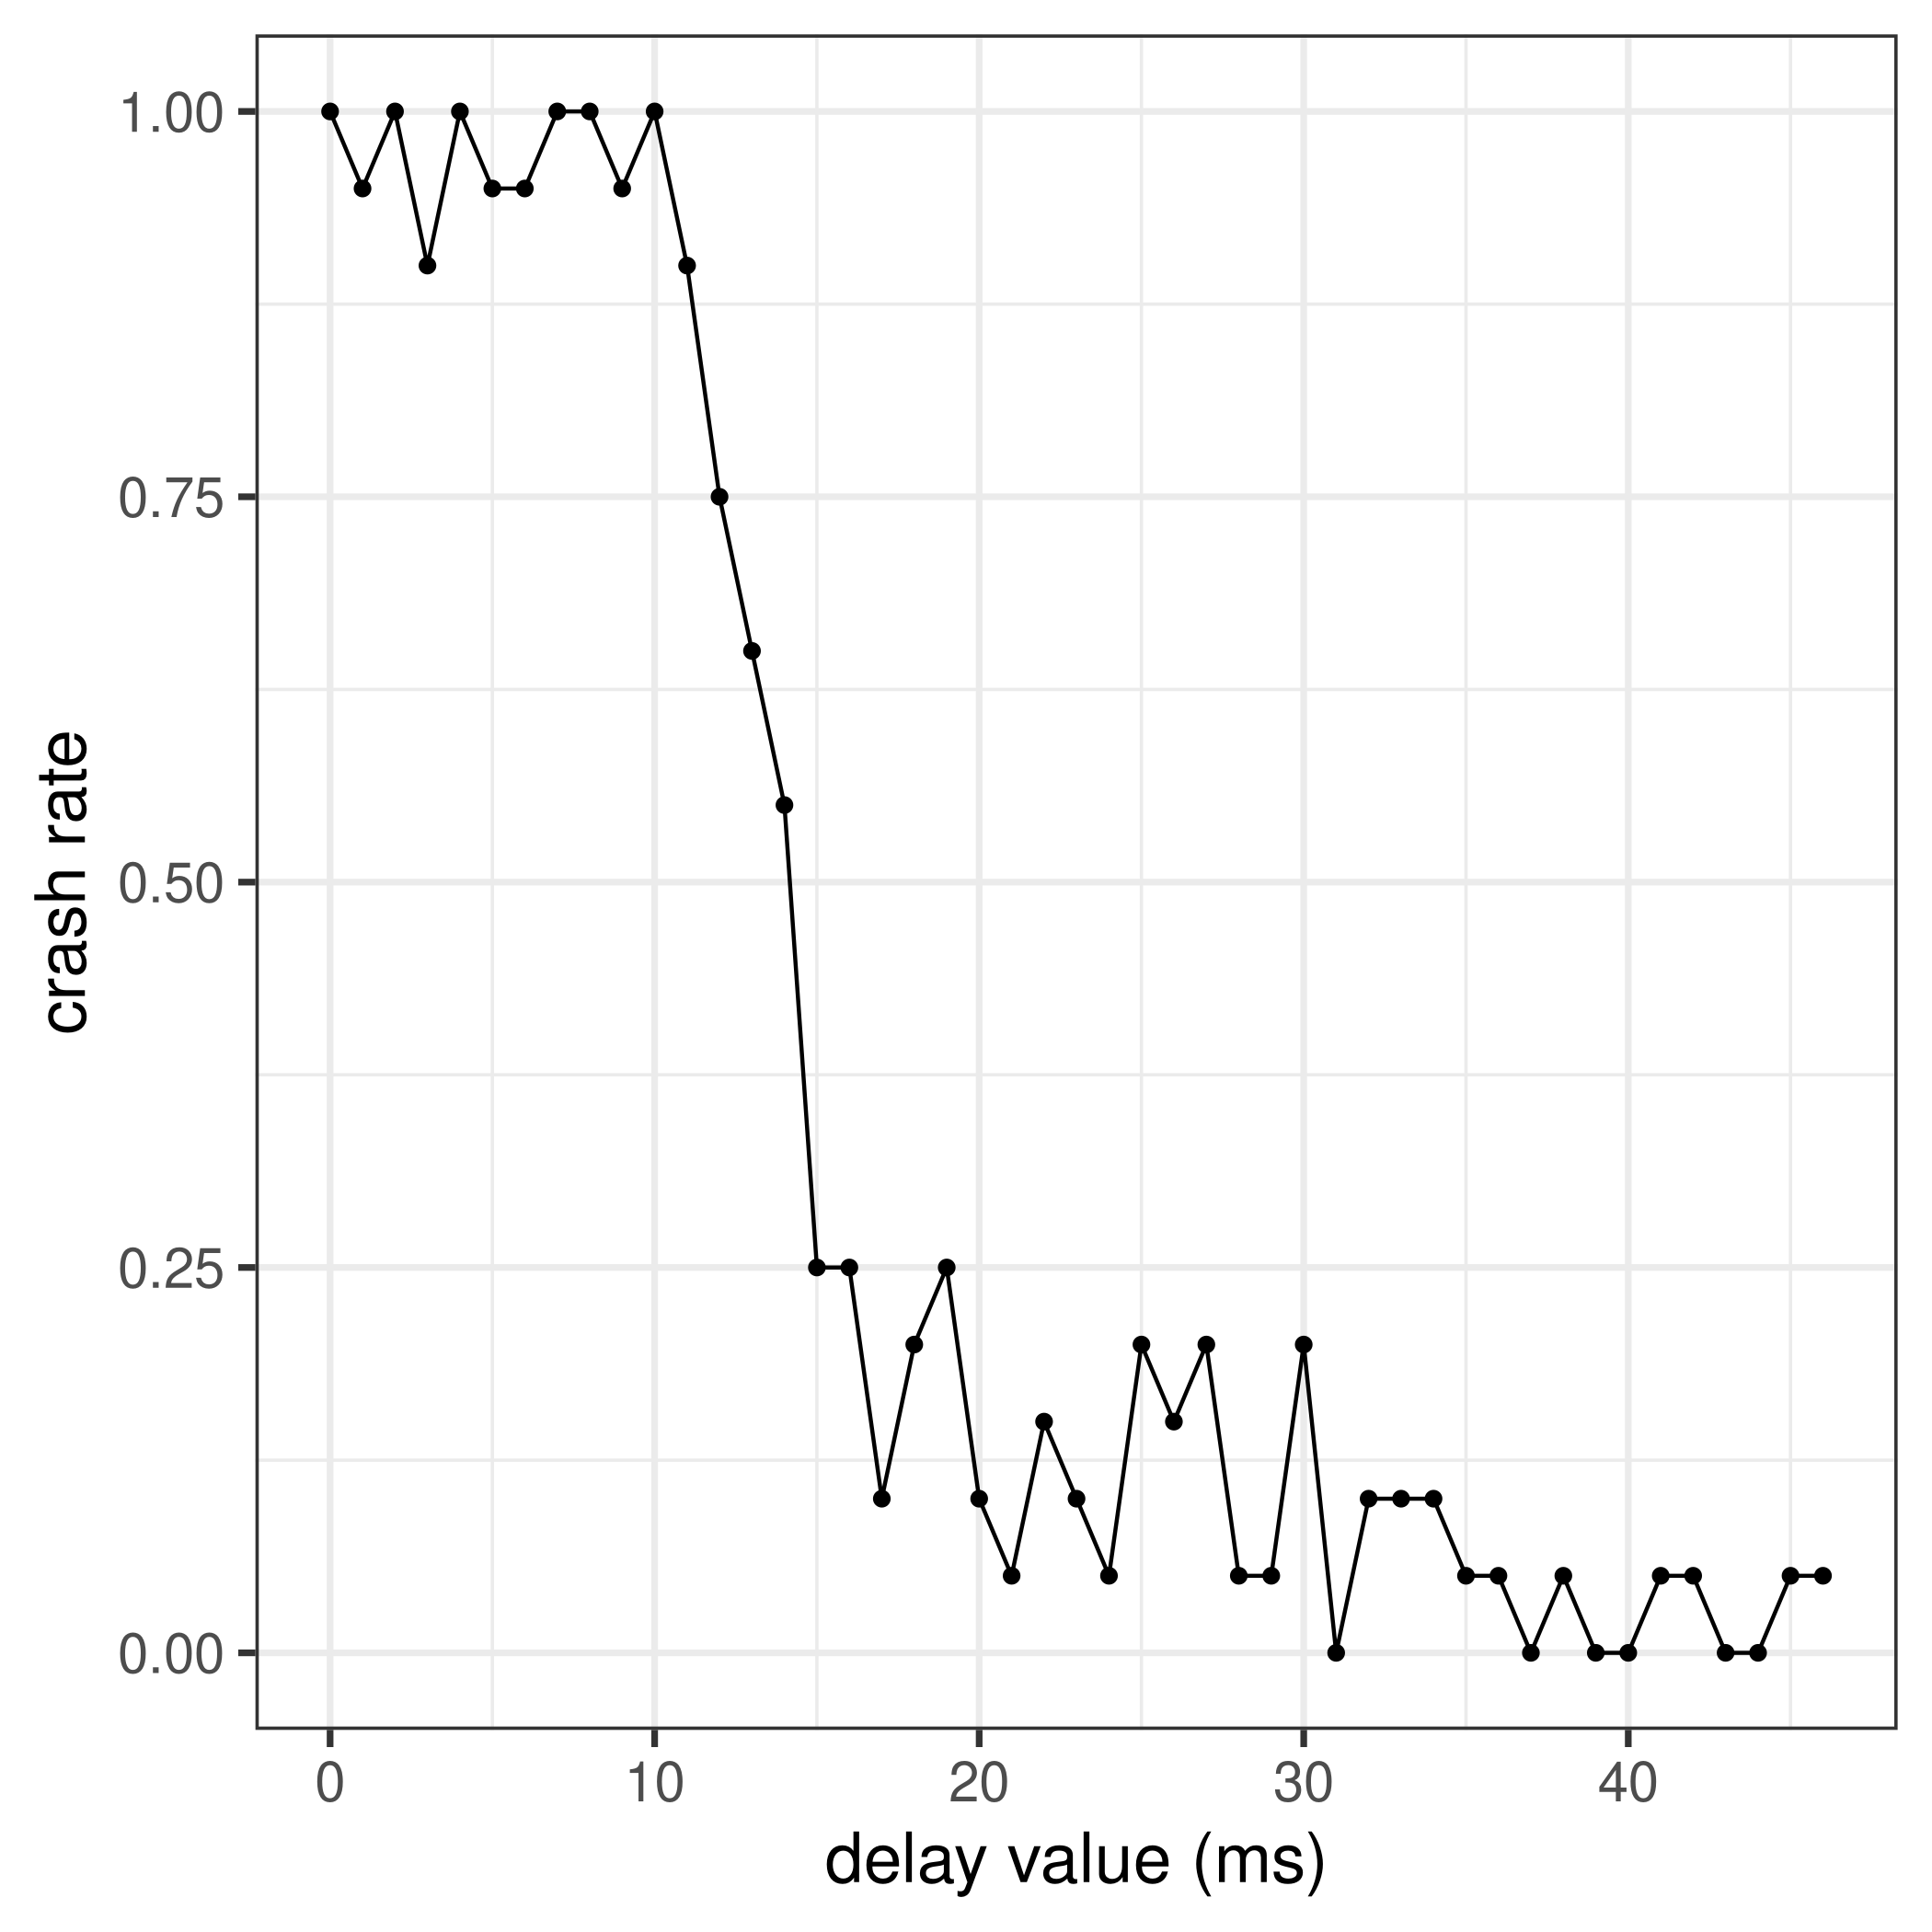
\includegraphics[scale=0.3]{../imgs/min-delay_crash_old.png}\\
	Note: inclure ce graphe?

	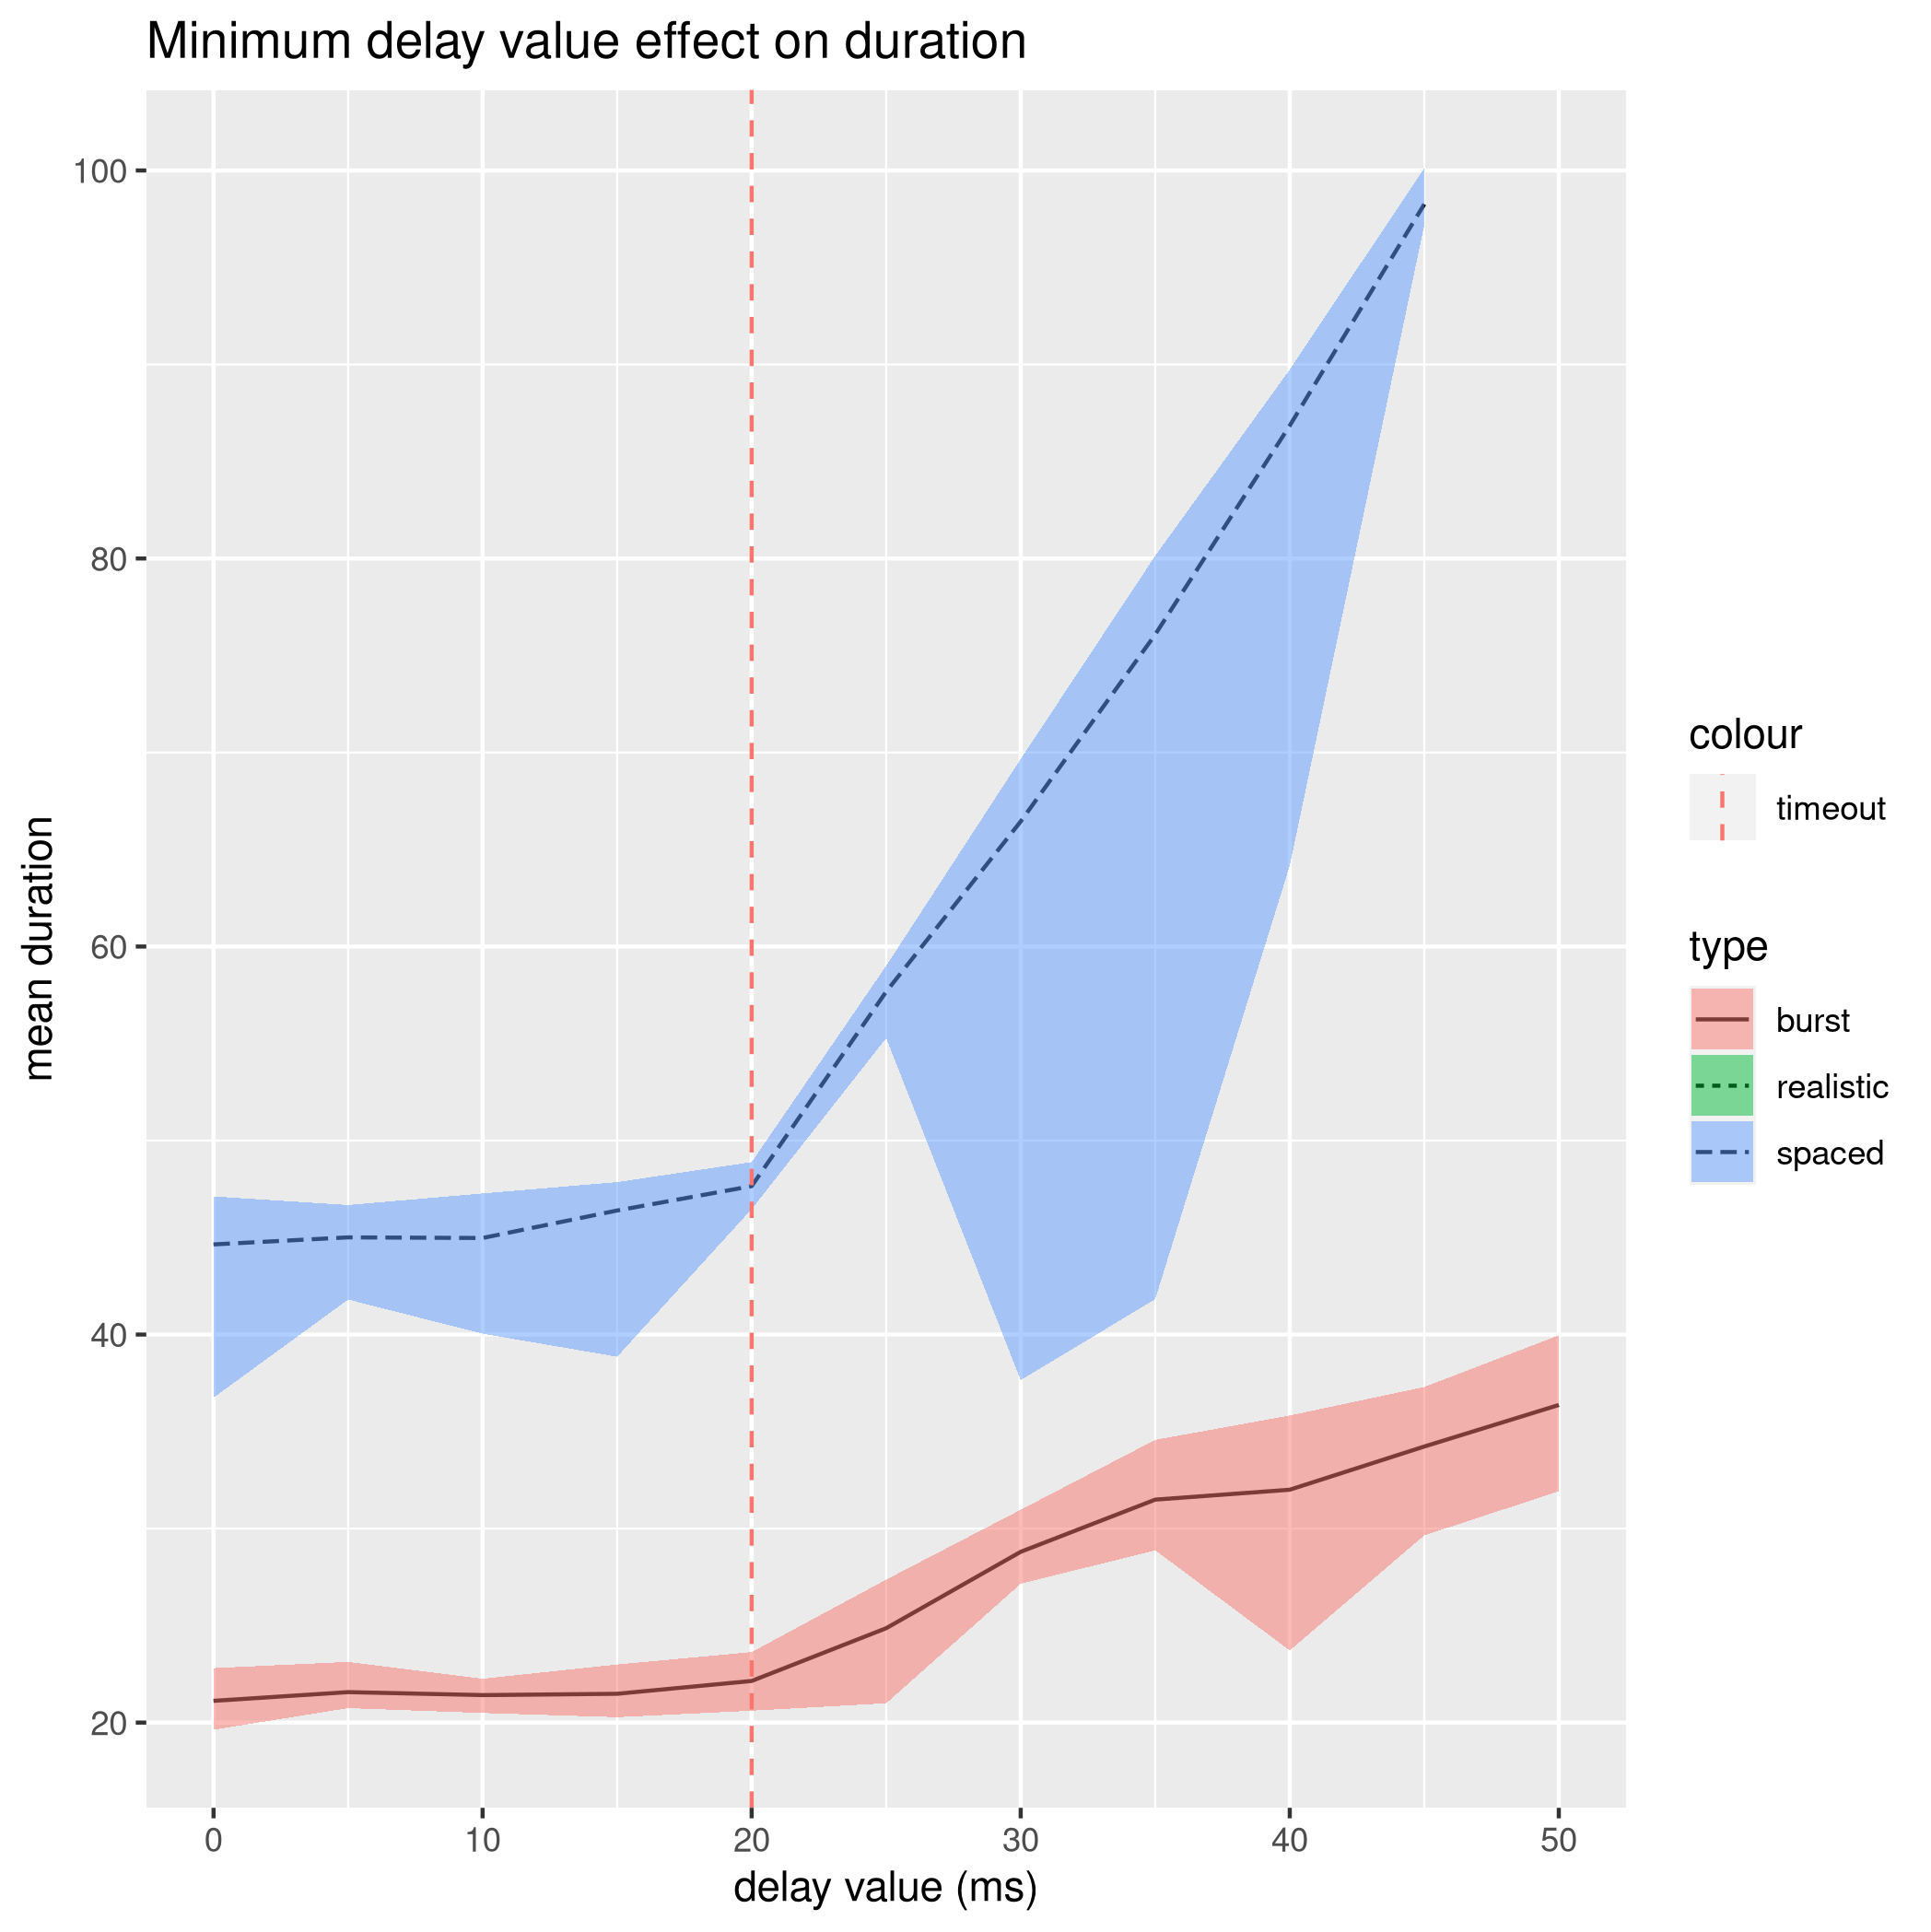
\includegraphics[width=\textwidth]{../imgs/min-delay_duration.png}
\end{frame}

\begin{frame}[allowframebreaks]{Timeout}
	\centering
	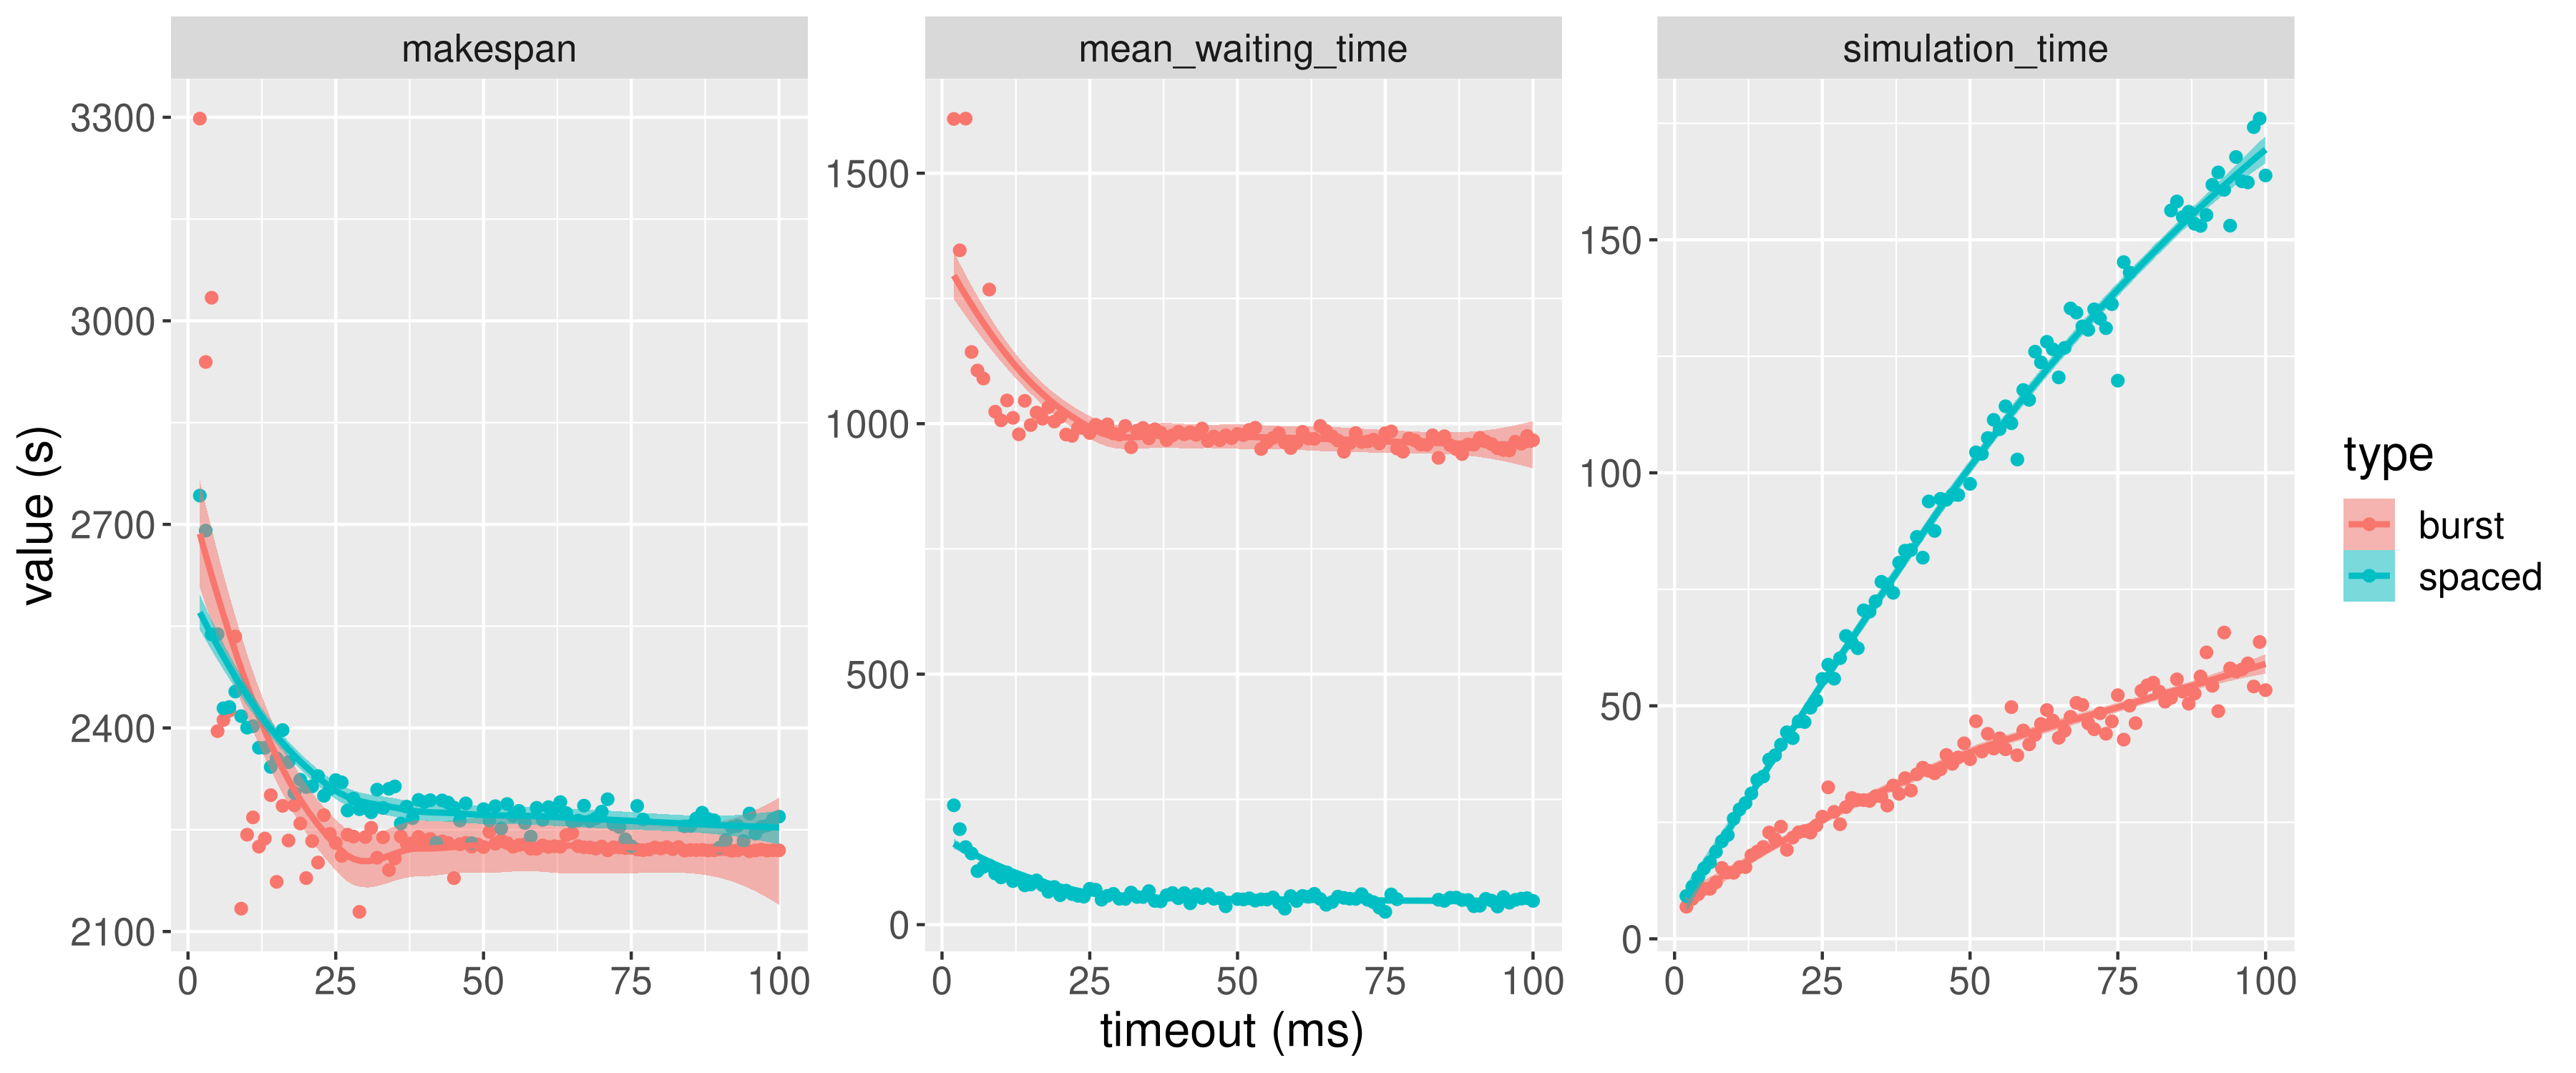
\includegraphics[width=\textwidth]{../imgs/timeout_burst_spaced.png}
	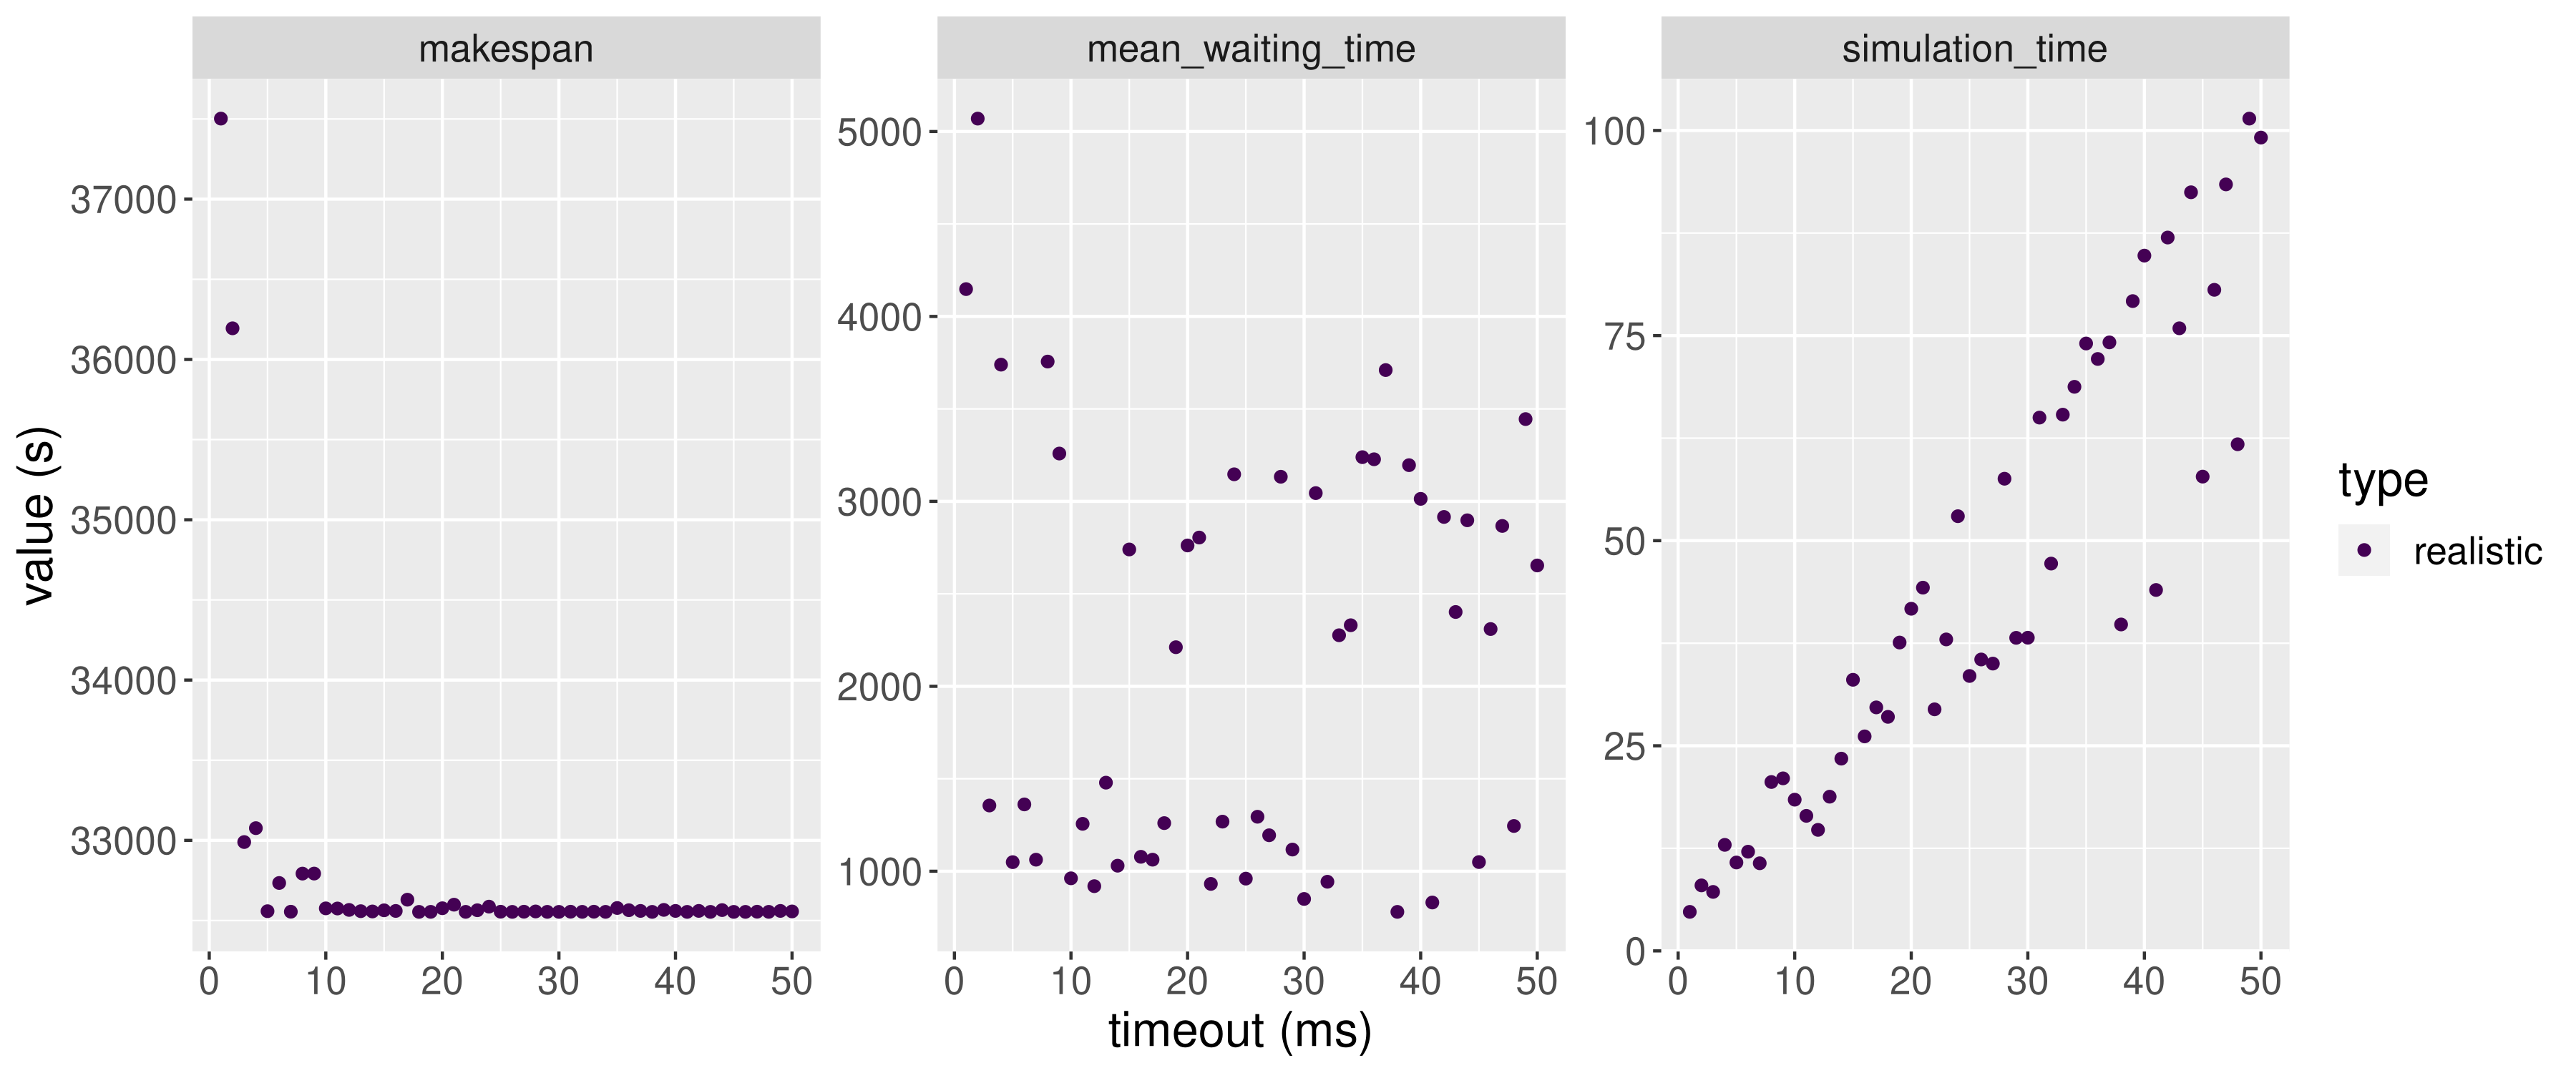
\includegraphics[width=\textwidth]{../imgs/timeout_realistic.png}
\end{frame}

\begin{frame}[allowframebreaks]{Maximum simulation timestep}
	\centering
	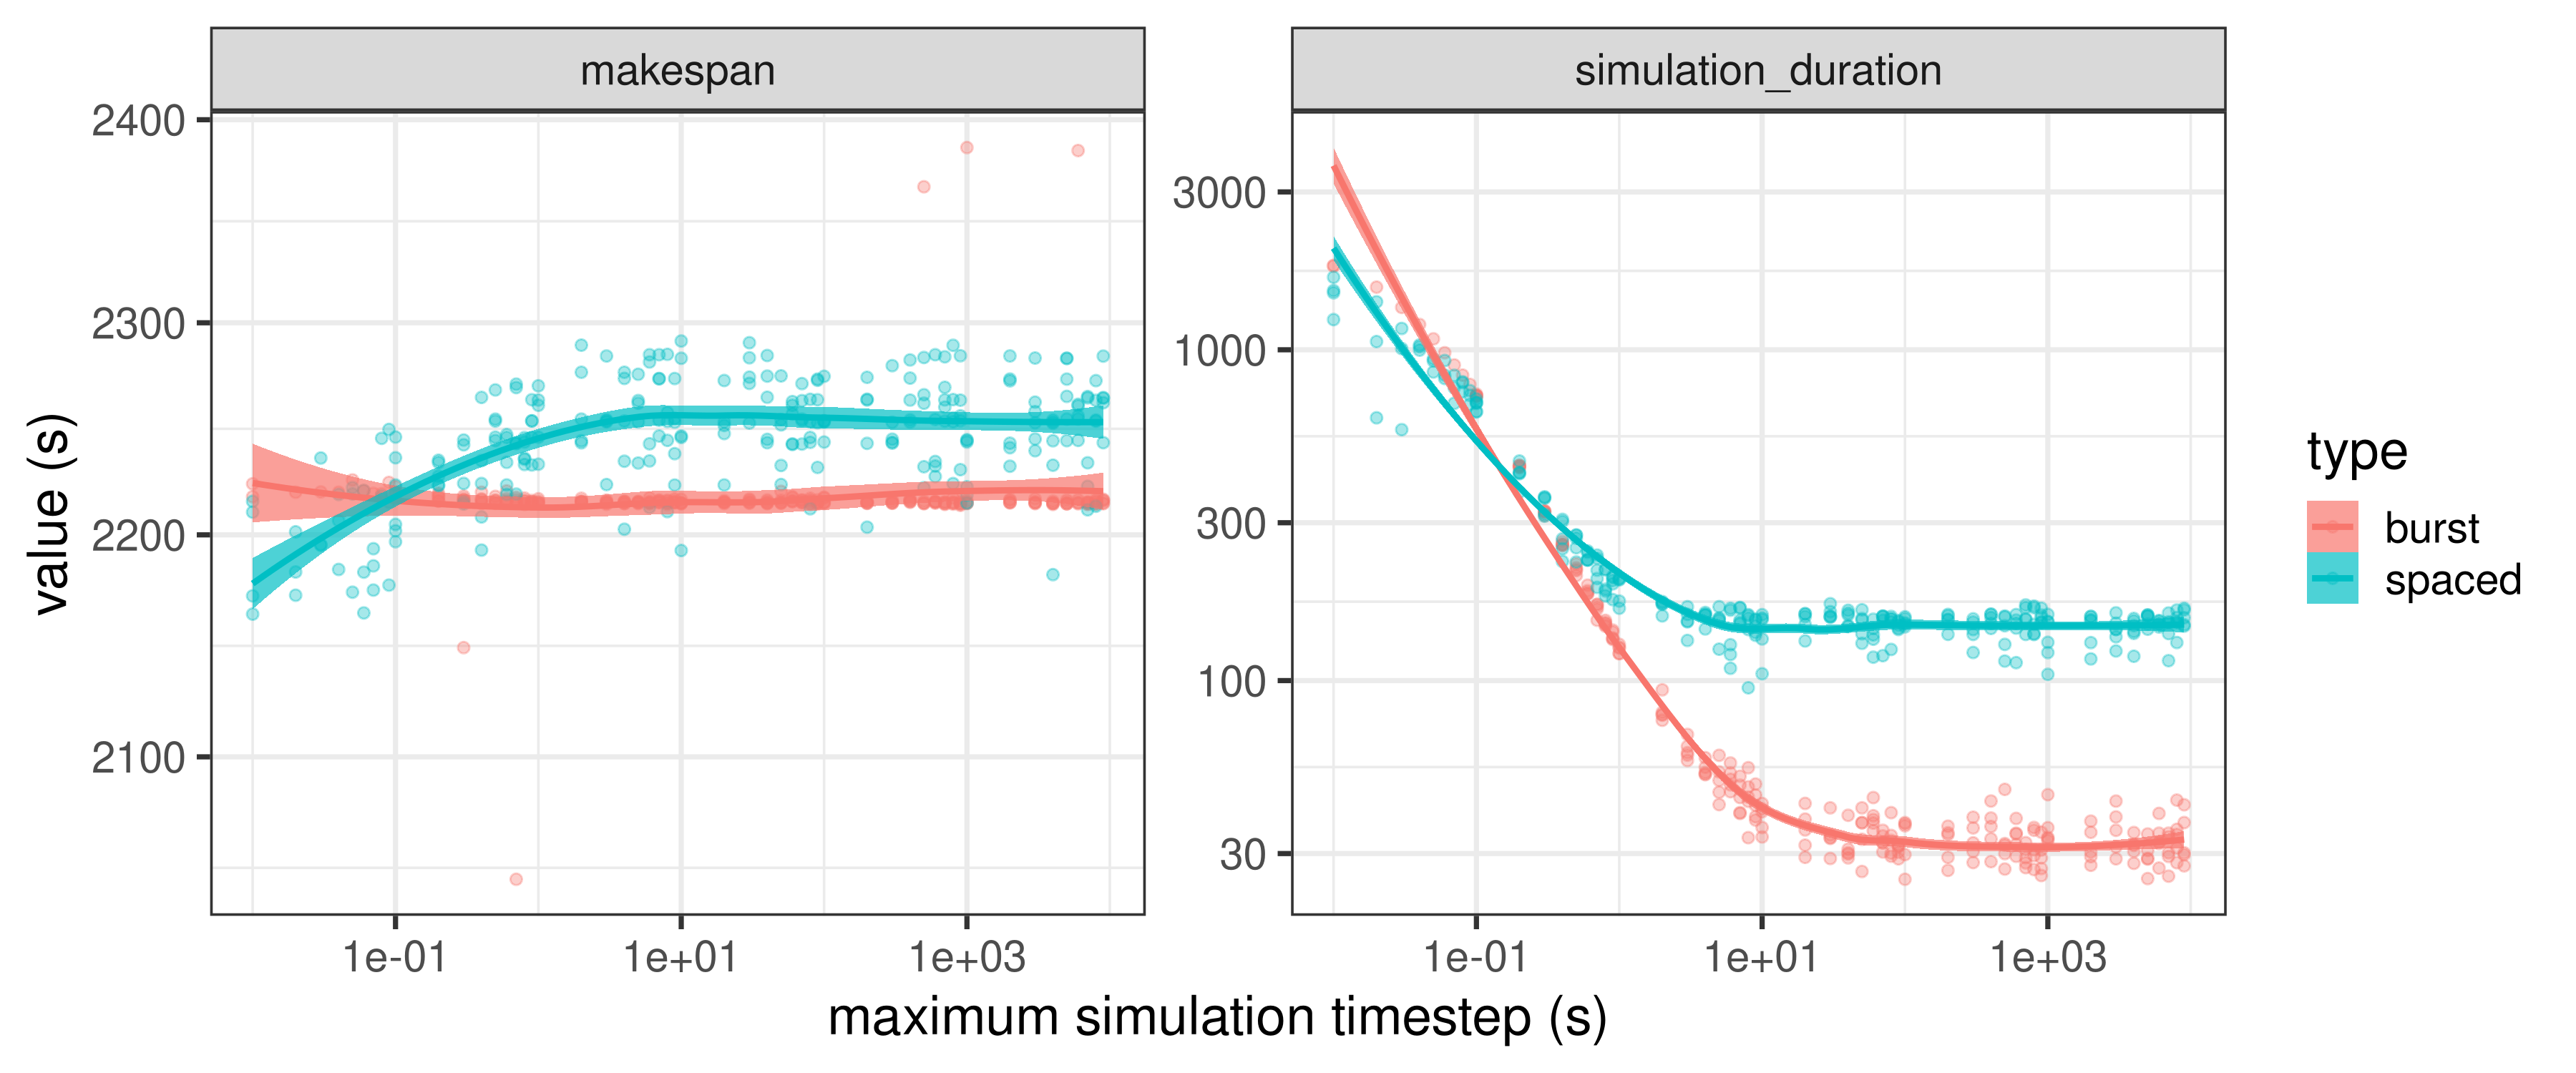
\includegraphics[width=\textwidth]{../imgs/max-timestep_burst_sp.png}
	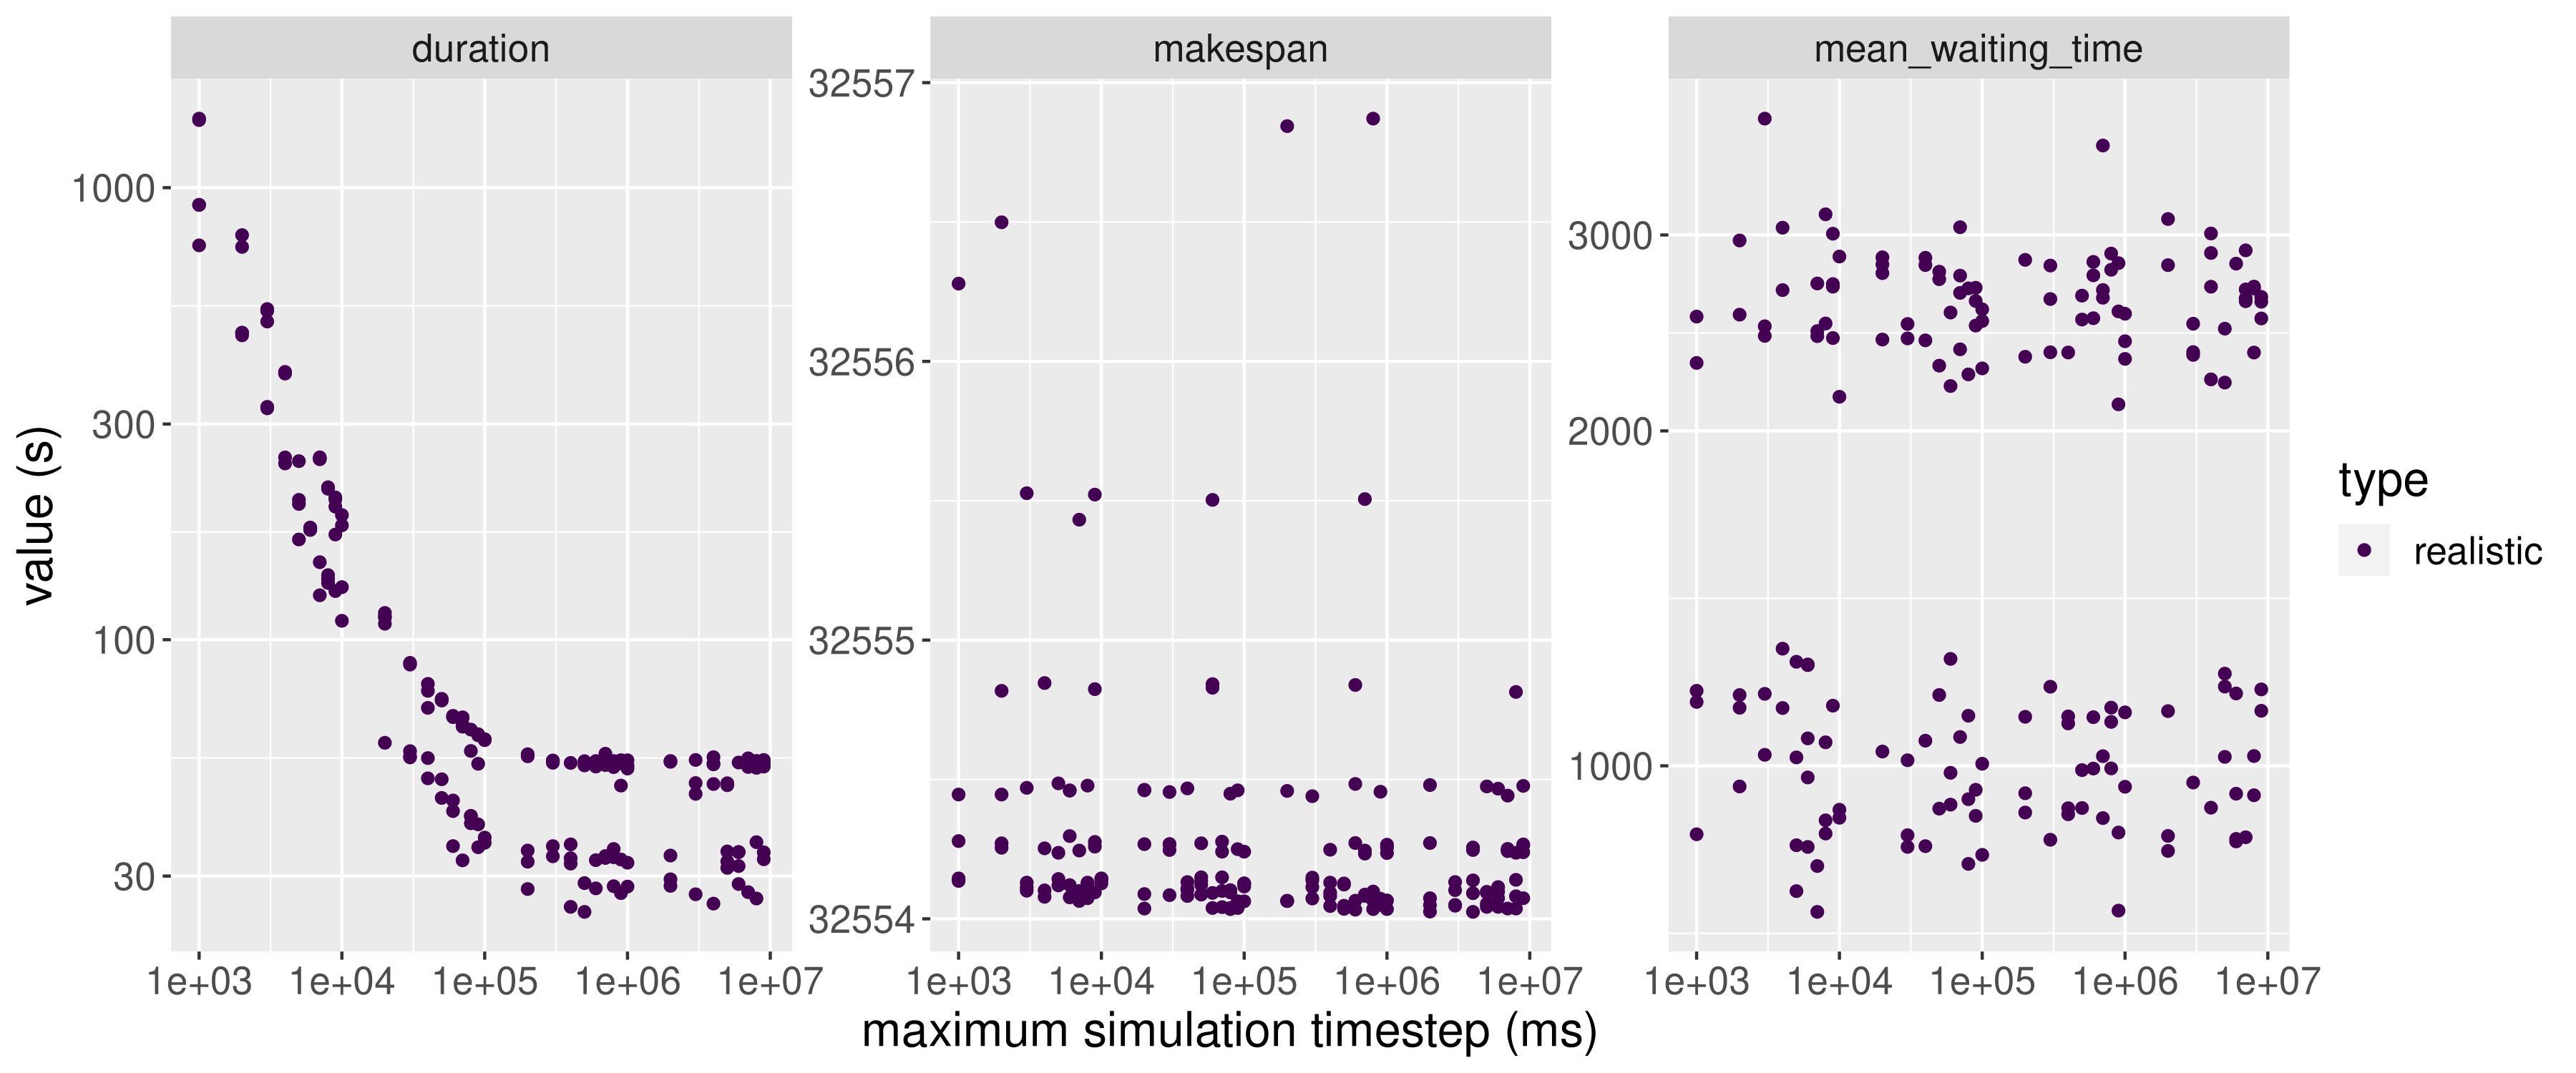
\includegraphics[width=\textwidth]{../imgs/max-timestep_realistic.png}
\end{frame}

\begin{frame}{Experimentation on a real cluster}
	\centering
	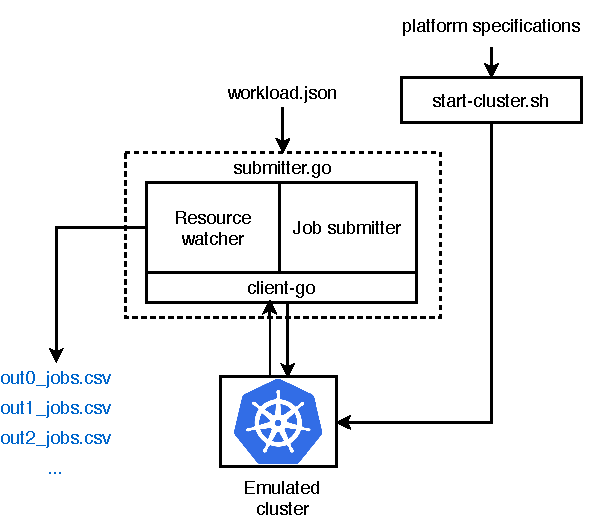
\includegraphics[width=0.8\textwidth]{../imgs/expe-protocole-v2.pdf}
\end{frame}

\begin{frame}{Deviation with reality}
	\centering
	\begin{adjustbox}{max width=\textwidth}
		\begin{tabular}{|c|c|c|c|c|c|c|c|c|}
			\hline

			\multirow{3}{*}{workload} & \multicolumn{4}{c|}{\textbf{makespan}} & \multicolumn{4}{c|}{\textbf{mean waiting time}}\\

			\cline{2-9}

			& \multicolumn{2}{c|}{emulated} &
			\multicolumn{2}{c|}{simulated} & \multicolumn{2}{c|}{emulated}
			& \multicolumn{2}{c|}{simulated} \\

			\cline{2-9}

			& $\mu$ & $\sigma$ & $\mu$ & $\sigma$ & $\mu$ & $\sigma$ & $\mu$ & $\sigma$ \\

			\hline

			burst & 2467 & 28.3 & 2215 (-252) & 0.508 & 1077 & 10.6 & 970 (-107) & 12.6 \\
			spaced & 2468 & 5.14 & 2257 (-211) & 16.9 & 146 & 1.67 & 48.1 (-97.9) & 9.44 \\
			realistic & 32556 & - & 32555 (-1) & 1.30 & 2884 & - & 2020 (-864) & 950 \\
			\hline
		\end{tabular}
	\end{adjustbox}
\end{frame}

\section{Discussion and future work}
\begin{frame}{Capabilities of Batkube}
	- delay jobs\\
	- cpu and memory requests\\
	- can patch any kubernetes scheduler written in Go\\
	- the api only supports the default scheduler
\end{frame}

\begin{frame}{Limitations}
	- memory hungry (in fact, the scheduler is memory hungry)\\
	- some problems with the scheduler\\
	- not scalable
\end{frame}

\begin{frame}{Perspectives for future work}
	- parallel jobs\\
	- storage\\
	- more complete api: support for more schedulers but also tools (monitoring tools)
\end{frame}

\begin{frame}[allowframebreaks]
        \frametitle{References}
	\printbibliography
\end{frame}

\end{document}

